% !TeX spellcheck = en_US
\documentclass{article}
\usepackage[english]{babel}
\usepackage[utf8]{inputenc}
\usepackage{fancyhdr}
\usepackage{xcolor}
\usepackage{lmodern}
\usepackage{listings}
\usepackage{amsmath}
\usepackage{graphicx}
\usepackage{amssymb}
\lstset{language=[90]Fortran,
	basicstyle=\ttfamily,
	keywordstyle=\color{blue},
	commentstyle=\color{green},
	morecomment=[l]{!\ }% Comment only with space after !
}

\usepackage{color}
\definecolor{deepblue}{rgb}{0,0,0.5}
\definecolor{deepred}{rgb}{0.6,0,0}
\definecolor{deepgreen}{rgb}{0,0.5,0}

% Default fixed font does not support bold face
\DeclareFixedFont{\ttb}{T1}{txtt}{bx}{n}{10} % for bold
\DeclareFixedFont{\ttm}{T1}{txtt}{m}{n}{10}  % for normal

% Python style for highlighting
\lstset{
	language=Python,
	basicstyle=\ttm,
	otherkeywords={self},             % Add keywords here
	keywordstyle=\ttb\color{deepblue},
	emph={__init__},          % Custom highlighting
	emphstyle=\ttb\color{deepred},    % Custom highlighting style
	stringstyle=\color{deepgreen},
	frame=tb,                         % Any extra options here
	showstringspaces=false            % 
}





\pagestyle{fancy}
\fancyhf{}
\lhead{Vincenzo Maria Schimmenti - 1204565}
\rhead{\today}
\rfoot{Page \thepage}
\lfoot{Exercise 5}
\title{%
	Information Theory and Computation \\
	Exercise  5}
\author{Vincenzo Maria Schimmenti - 1204565}
\begin{document}
\maketitle
 
\section*{Theory and requests}
In this assignment we are going to study the behavior of the eigenvalues of random Hermitian matrices; denote $\{ \lambda_i \}_{i=1}^N$ the ordered set of these eigenvalues (which, by the spectral theorem, are real). We are interested in studying the normalized spacing:
\begin{equation}
	s_i = \frac{\lambda_{i+1}-\lambda_i}{\Delta \lambda}
\end{equation}
where $\Delta \lambda$ is the average $\Delta \lambda_i$. This average difference can be either compted \textit{globally}, considering all eigenvalues at once, or \textit{locally}, by computing an average difference for each eigenvalue, considering only some neighbors eigenvalues. We know (from Wigner) that the normalized spacing follows the following distribution:
\begin{equation}
	P(s)=2 \left(\frac{4s}{\pi}\right)^2 e^{-\frac{4s^2}{\pi}}
\end{equation}
Actually this expression is exact for $2 \times 2$ hermitian matrices and a good approximation for the bigger cases. We are exploit to use this functional form and fit the data we will obtain using:
\begin{equation}
	P(s)=a s^{\alpha} e^{-bx^\beta}
\end{equation}
The entries of the matrix are gaussian; the gaussian distributed numbers are obtained using the so called Box Muller distribution. Starting from a couple $(U,V)$ of uniform random variables in $[0,1]$ we have the the two variables $Z_1$ and $Z_2$ are distributed (and independent) as $\mathcal{N}(0,1)$ if:
\begin{flalign}
	& Z_1=\sqrt{-2\ln U} \cos(2\pi V) \\
	& Z_2 = \sqrt{-2\ln U} \sin(2\pi V)
\end{flalign}
We are also required to the report the average of
\begin{equation}
	r_i = \frac{\min(\Delta \lambda_i,\Delta \lambda_{i+1})}{\max(\Delta \lambda_i, \Delta \lambda_{i+1})}
\end{equation}
\section*{Code Development}
After we generated the random matrix $H$ of size $N \times N$ (which is a parameter of the program), we use the Lapack subroutine \textit{cheev} to diagonalize it:
\begin{lstlisting}[language=Fortran]
call cheev('N','U',nn,matr,nn,eigvs,work,lwork,rwork,info)
\end{lstlisting}
The character N tells Lapack to returns only the eigenvalues, U tells to use the upper diagonal part of the matrix (since is hermitian we can choose); the eigenvalues are stored inside the vector \textit{eigvs}. Actually before being able to properly diagonalize the matrix, one has to tweak an internal parameter of the subroutine by calling it with \textit{lwork=-1}.
\begin{lstlisting}[language=Fortran]
! optimal lwork
lwork=-1
allocate(work(1))
allocate(rwork(max(1, 3*nn-2)))
if(.not.allocated(eigvs))allocate(eigvs(nn))
call cheev('N','U',nn,matr,nn,eigvs,work,lwork,rwork,info)
lwork = int(real(work(1)))
deallocate(work)
deallocate(rwork)
! actual diag
allocate(work(max(1,lwork)))
allocate(rwork(max(1, 3*nn-2)))
call cheev('N','U',nn,matr,nn,eigvs,work,lwork,rwork,info)
\end{lstlisting}
If the diagonalization goes well (i.e. the parameter \textit{info} is zero), we compute the difference between the eigenvalues and normalize according to the given prescription (global or local average, as above explained); during this step we also compute and save the values $r_i$'s. Having the spacings, we order them (using a merge-sort) and we create an histogram from them, according to a fixed cutoff (i.e. biggest value of the spacing to be considered in the binning procedure)  and to a given number of bins. The Fortran program stops here by saving the obtained histogram. This whole procedure is done multiple times in order to sample different matrices, then a python script handles the fitting procedure using the fucntion described in the previous section.
\newpage
\section*{Results}
We used $2000 \times 2000$ matrices with $150$ sampled matrices; we also used $300$ bins for the histogram with a cutoff equals to $3.5$, which retains the $99\%$ of the spacings. As mentioned earlier, we also computed the histogram both using the global and local mean and for diagonal and general hermitian matrices. In the following table the results of the fit and the average $r_i$ are shown:
\begin{center}
	\begin{tabular}{|c|c|c|c|c|}
		\hline 
		& Global & Local & Global Diag & Local Diag \\ 
		\hline 
		a & 11.90 & 3.77 & 1.23 & 1.12  \\ 
		\hline 
		$\alpha$ & 2.48  & 2.02 & $\approx 0$  & $\approx 0$  \\ 
		\hline 
		b & 2.67 & 1.45  &  1.11 & 1.11  \\ 
		\hline 
		$\beta$ & 1.36  & 1.86  & 1.17 & 1.05 \\ 
		\hline
		$\langle r \rangle$ & 0.60 & 0.60 & 0.39 &  0.39\\
		\hline
	\end{tabular} 
\end{center}
Here instead we show the density from the data, the fitted one and, in case of general matrices, the theoretical one.
\begin{center}
	\begin{figure}[h!]
		\begin{tabular}{cc}
			Global & Local \\
			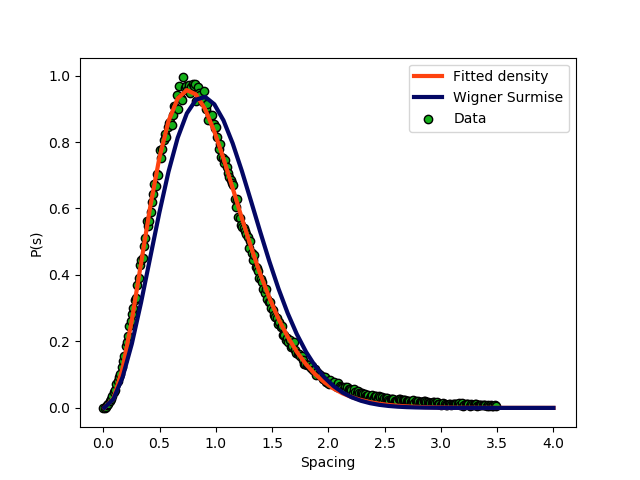
\includegraphics[width=0.5\linewidth]{pdf_2000_150_300_0_0.png} &
			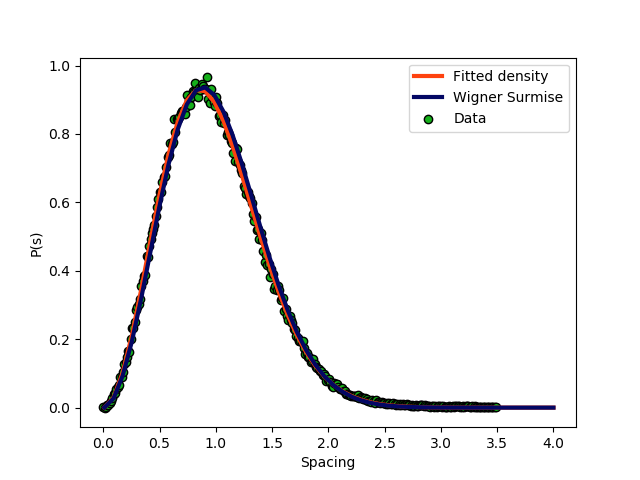
\includegraphics[width=0.5\linewidth]{pdf_2000_150_300_0_1.png} \\
			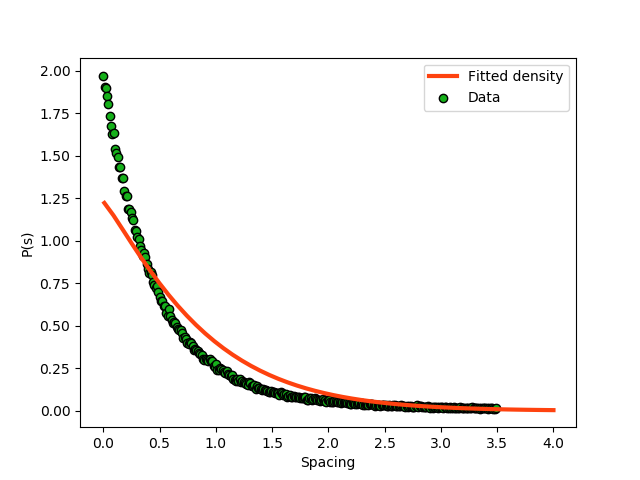
\includegraphics[width=0.5\linewidth]{pdf_2000_150_300_1_0.png} &
			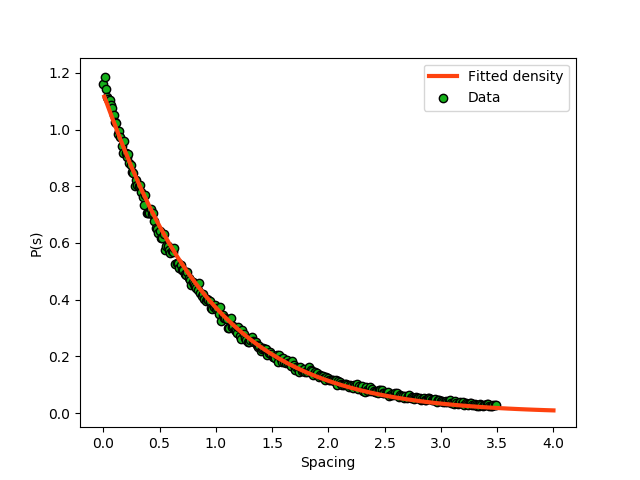
\includegraphics[width=0.5\linewidth]{pdf_2000_150_300_1_1.png} \\
		\end{tabular}
		\caption{The first rows represent general hermitian matrices, the second the diagonal ones.}
	\end{figure}
\end{center}
We notice how using local averages instead of the global ones the data follows more accurately the theoretical distribution (in the case of general matrices).
\section*{Info}
If one wants to launch the program the following is the argument list: \\
\textbf{./eigenproblem.out \textit{size} \textit{nSamples} \textit{nBins} \textit{mode} \textit{avgMode}} \\
where mode=0,1 stands for general or diagonal and avgMode=0,1 for global or local average of spacings.
The same goes for the python script:\\
\textbf{python eigenproblem.py \textit{size} \textit{nSamples} \textit{nBins} \textit{mode} \textit{avgMode}} \\
%(0,0)
% Parameters: [11.89906761  2.47844214  2.67535329  1.36231397]
%0.5995035633126873 +/- 0.00671548720225846

%(0,1)
%Parameters: [3.77371651 2.02558911 1.449321   1.86130905]
%0.9986180543399098 +/- 2.2107482086263488e-05



%(1,0)
%Parameters: [1.22837607e+00 7.92094572e-08 1.11527368e+00 1.17597899e+00]
%0.3860044305197628 +/- 0.007372506743899098

%(1,1)
%Parameters: [1.12579060e+00 7.93108879e-09 1.10672584e+00 1.04850414e+00]
%0.9965524254667237 +/- 0.00010919142898528652




\end{document}